\documentclass[aspectratio=169, 8pt, xcolor={svgnames}]{beamer}
\usetheme[progressbar=frametitle]{metropolis}
\setbeamercolor{background canvas}{bg=white}
\setbeamerfont{footnote}{size=\tiny}
\usepackage{hyperref}

% Impostazioni per il colore dei link
\hypersetup{
    colorlinks=true,    % Attiva i colori per i link
    linkcolor=black, % Colore dei link interni
    urlcolor=persianred        % Colore dei link esterni (url)
}
\usepackage{appendixnumberbeamer}
\usepackage{url}
\usepackage{amsfonts} 
\usepackage{amssymb}
\usepackage[english]{babel}
\usepackage{fontawesome}
\usepackage{multicol}
\usepackage{braket}
\usepackage{overpic} 
\usepackage{bm}
\usepackage{braket}
\usepackage{algorithm}
\usepackage{algpseudocode}
\usepackage{enumitem}

\usepackage[]{pseudo}

\usepackage{tikz}
\usetikzlibrary{positioning,arrows,calc,math,angles,quotes}
\usepackage{blochsphere}

\usetikzlibrary{arrows,automata}
\usetikzlibrary{positioning}
\usetikzlibrary{arrows.meta,
                bending,
                intersections,
                quotes,
                shapes.geometric}

\tikzset{
    state/.style={
           rectangle,
           rounded corners,
           draw=black, very thick,
           minimum height=1em,
           inner sep=2pt,
           text centered,
           },
}

\definecolor{myv}{rgb}{0.36, 0.22, 0.33}
\definecolor{gio}{rgb}{0.45, 0.31, 0.59}
\definecolor{light}{rgb}{0.8, 0.8, 1}
\definecolor{warmblack}{rgb}{0.0, 0.26, 0.26}
\definecolor{brown(web)}{rgb}{0.65, 0.16, 0.16}
\definecolor{cadmiumgreen}{rgb}{0.0, 0.42, 0.24}
\definecolor{darkmidnightblue}{rgb}{0.0, 0.2, 0.4}
\definecolor{brightube}{rgb}{0.82, 0.62, 0.91}
\definecolor{bleudefrance}{rgb}{0.19, 0.55, 0.91}
\definecolor{brightmaroon}{rgb}{0.76, 0.13, 0.28}
\definecolor{codegreen}{rgb}{0,0.6,0}
\definecolor{codegray}{rgb}{0.5,0.5,0.5}
\definecolor{codepurple}{rgb}{0.58,0,0.82}
\definecolor{backcolour}{rgb}{0.95,0.95,0.92}
\definecolor{amethyst}{rgb}{0.6, 0.33, 0.73}
\definecolor{mediumpersianblue}{rgb}{0.0, 0.4, 0.65}
\definecolor{persianred}{rgb}{0.8, 0.2, 0.2}
\definecolor{deepcarrotorange}{rgb}{0.91, 0.41, 0.17}

\usepackage[most]{tcolorbox}
\usepackage{xcolor}


\title{Boosting ground states preparation with double-bracket quantum algorithms}
\subtitle{\texttt{PART 1:} Introducing and optimizing double-bracket quantum algorithms}
\date{28 November 2024}
\author{Matteo Robbiati}
\titlegraphic{
   \begin{tikzpicture}[overlay, remember picture]
   \node[at=(current page.south east), anchor=south east] {%
      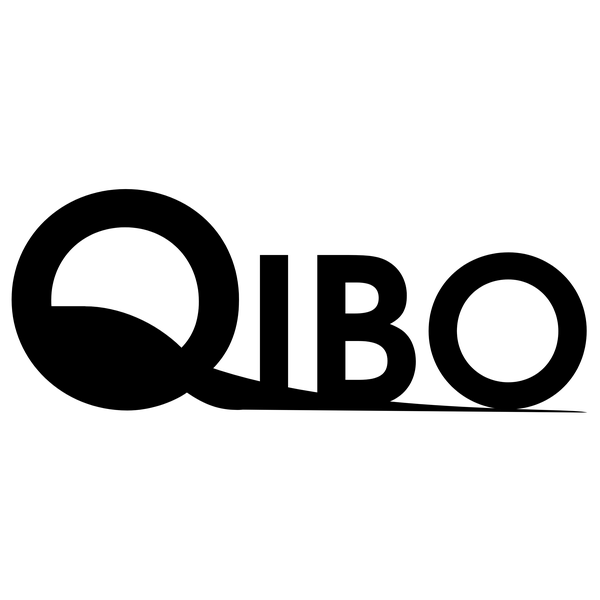
\includegraphics[width=.15\textwidth]{figures/qibo.png} 
      
\includegraphics[width=.15\textwidth]{figures/unimi.png} 
      
\includegraphics[width=.15\textwidth]{figures/cern.png}  
      
\includegraphics[width=.15\textwidth]{figures/qti.png}  
   };
   \end{tikzpicture}
}

\begin{document}

\begin{frame}
\maketitle
\end{frame}

\begin{frame}{A couple of references}
\begin{multicols}{2}
\begin{figure}
   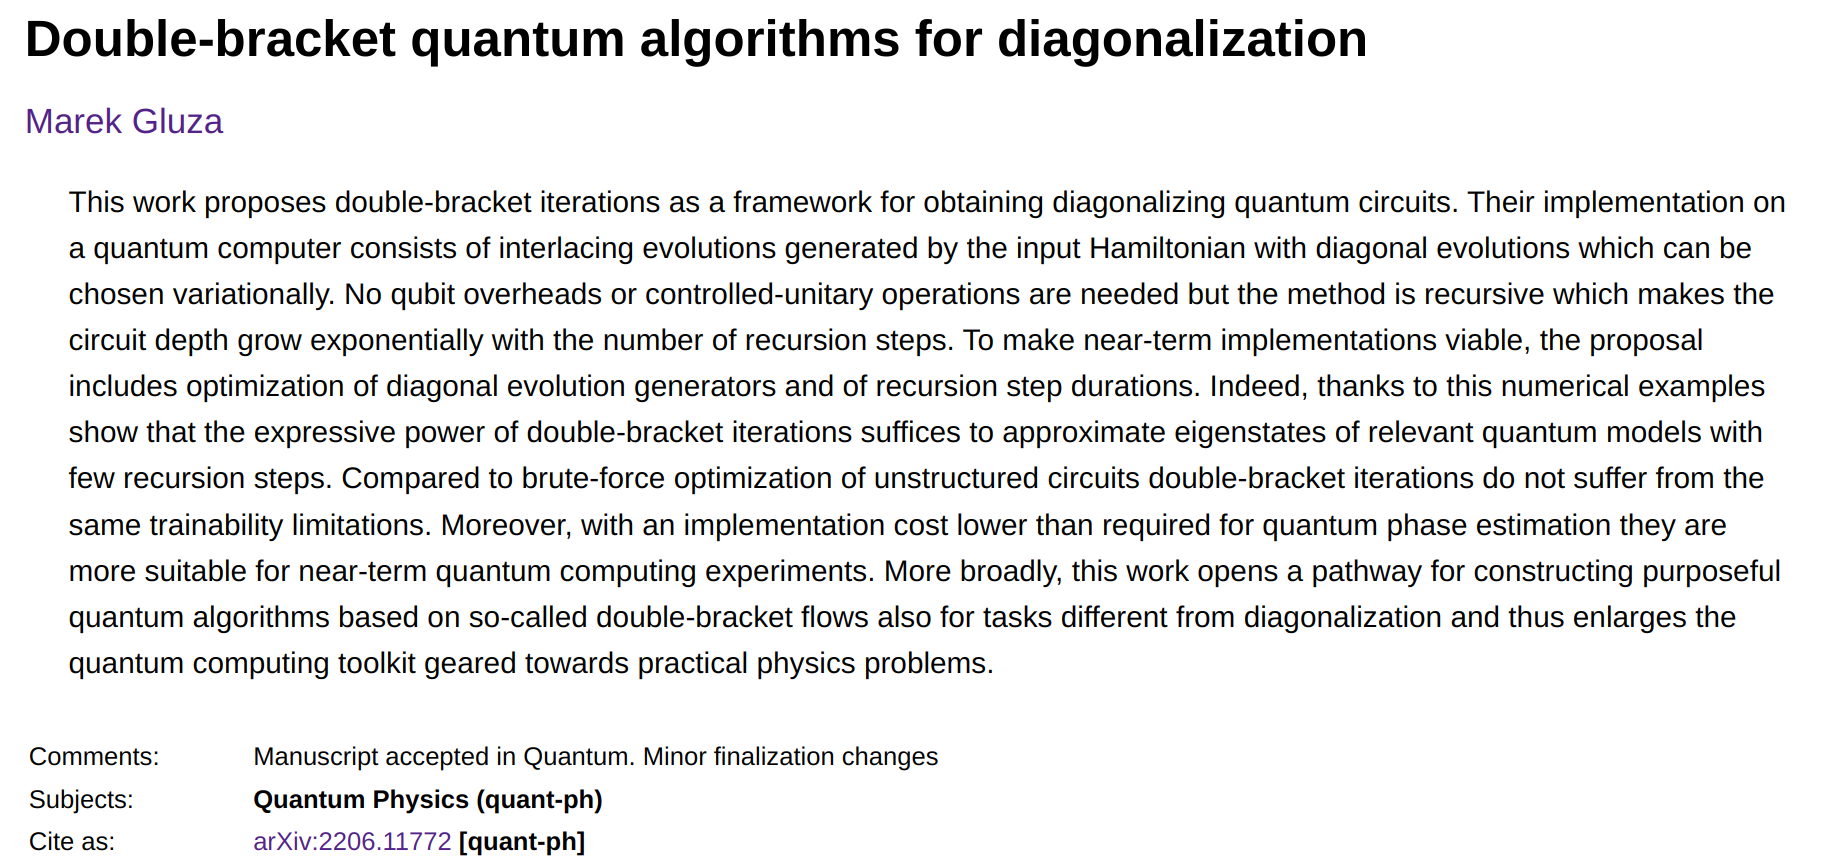
\includegraphics[width=0.5\textwidth]{figures/dbqa_paper.png}
\end{figure}
Check out this because:
\begin{itemize}[noitemsep]
\item[1.] Marek is a very nice and smart guy;
\item[2.] it contains math foundations of this talk; 
\end{itemize}
\begin{figure}
   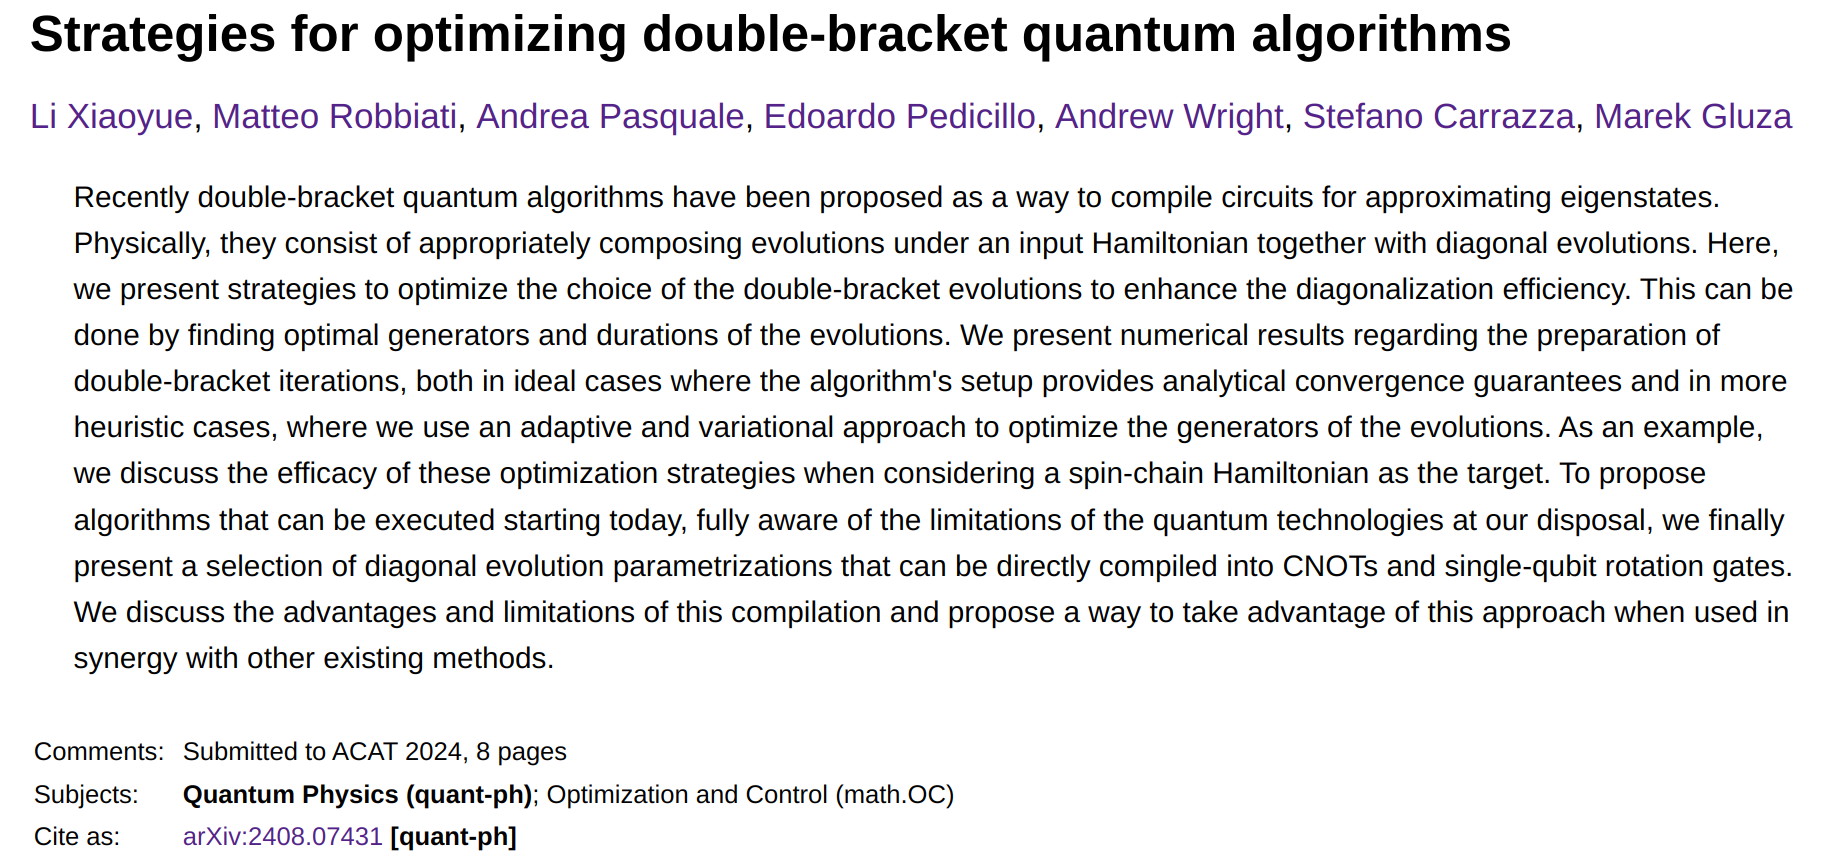
\includegraphics[width=0.5\textwidth]{figures/dbqa_opt.png}
\end{figure}
And this because:
\begin{itemize}[noitemsep]
\item[1.] We delve deeper into the optimization of DBQAs;
\item[2.] we base the optimization of the next talk on these studies. 
\end{itemize}
\end{multicols}
\end{frame}

\begin{frame}{Double-bracket iterations \hfill \href{https://arxiv.org/abs/2206.11772}{\textcolor{white}{\faBook\,\,arXiv:2206.11772}}}
\begin{columns}[T,onlytextwidth]
    % First column: 40%
    \begin{column}{0.45\textwidth}
    \textbf{Ingredients}
        \begin{itemize}[noitemsep]
            \item[1.] Input Hamiltonian $\textcolor{mediumpersianblue}{\hat H_0}$ (here 1D XXZ);
            \item[2.] an anti-hermitian ($(i\hat{W})^{\dagger} = -i\hat{W}$) rotation generator $\textcolor{persianred}{\hat{W}_0} = [\hat{D}_0, \hat H_0]$;
            \item[3.] point 2. is used to build a unitary operation:
              $$ \hat{R}_0 \equiv e^{s \textcolor{persianred}{\hat{W}_0}}, $$
              with $s$ stepsize or flow duration;
            \item[4.] $\hat{R}_0$ applied to $\hat{H}_0$ as \textit{double-bracket rotation}:
               $$ \hat H_1 =  e^{s\textcolor{persianred}{\hat{W}_0}} \textcolor{mediumpersianblue}{\hat H_0} e^{- s \textcolor{persianred}{\hat{W}_0}}.$$
        \end{itemize}

    \end{column}

    % Second column: 60%
    \begin{column}{0.55\textwidth}
        \begin{figure}
           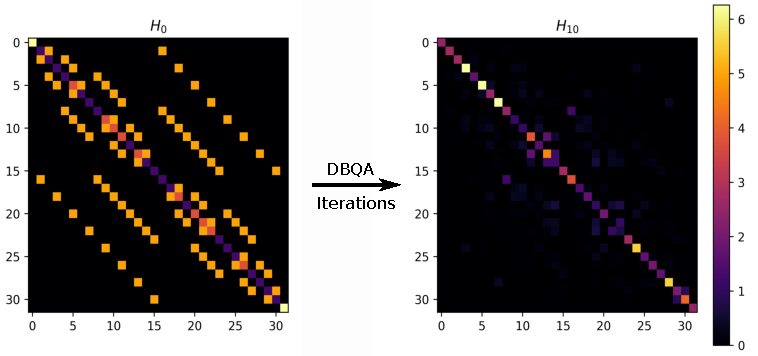
\includegraphics[width=0.95\textwidth]{figures/dbqa_10steps.pdf}
        \caption{Ten DBQA rotations to a 5 qubit 1D XXZ.}
        \end{figure}
    \end{column}
\end{columns}
\begin{tcolorbox}[colback=red!15, title=Nomenclature reason]
The presented framework satisfies a Heisenberg equation involving two, not one, brackets:
$$ \partial_s \hat{H}_0(s) = [ \hat{H}_0(s), [ \hat{H}_0(0), \hat{D}_0 ] ]. $$
\end{tcolorbox}
\end{frame}

\begin{frame}{Some properties and important notes \hfill \href{https://arxiv.org/abs/2206.11772}{\textcolor{white}{\faBook\,\,arXiv:2206.11772}}}
\begin{itemize}[noitemsep]
\item[1.] We care of diagonal 
   $\hat{D}_k$ in $\hat{W}_k = [\hat{D}_k, \hat{H}_k]$. A natural choice is the canonical
   generator:
   $$ 
   \hat{W}_k^{\rm can} = [\hat{H}_k, \hat{\Delta}(\hat{H}_k)], \qquad \text{with} \qquad  
   \begin{cases}
   \hat{\Delta}(\hat{H}_k) = \text{diag}(\hat{H}_k), \\
   \hat{H}_k = \hat{\Delta}(\hat{H}_k) + \hat{\sigma}(\hat{H}_k),
   \end{cases}
   $$
   but - as we will see - many choices can be done here.
\item[2.] \textbf{Lemma}\footnote{Definition and proof of Lemma 2 in \href{https://arxiv.org/abs/2206.11772}{Double-bracket 
   quantum algorithms for diagonalization, M. Gluza, 2024}}: given $\sigma(\hat{H}_0(s))$ off-diagonal restriction of $\hat{H}_0(s)$ and
   $s$ small enough:
   $$ \partial_s \| \sigma(\hat{H}_0(s)) \|^2_{\rm HS} = - 2 \braket{ \hat{W}_0, 
   [\hat{H}_0, \sigma(\hat{H}_0(s))] }_{\rm HS}. $$ 
\item[3.] If $\hat{D}_0 = ... = \hat{D}^*$, as long as $s_0 = ... = s^*$
   are sufficiently small and $\hat{D}^*$ non degenerate, the recursion converges to a fixed point $\hat{H}_{\infty}$
   with $[\hat{H}_{\infty}, \hat{D}^*]$\footnote{\textbf{If you are really brave:} 
   \href{https://link.springer.com/book/10.1007/978-1-4471-3467-1}{Optimization and Dynamical Systems [Ch. 2.3], Uwe Helmke , John B. Moore, 1994.}}; 
\end{itemize}
\begin{tcolorbox}[colback=red!15]
\begin{itemize}[noitemsep]
\item[$2. \to$] If $\hat{D}_0$ is diagonal, then $\hat{H}_1$ will be more diagonal than $\hat{H}_0$,
\item[$3. \to$] the discrete DBI can converge arbitrary well,
\item[$3. \to$] \textit{analytically motivated} methods work in some setups but they can be slow.
\end{itemize}
\end{tcolorbox}
\begin{picture}(0,0)
    \put(325,30){
        
\includegraphics[width=0.12\textwidth]{figures/take_away.png}
    }
\end{picture}
\end{frame}

\begin{frame}{Cost functions and parametrization strategies \hfill \href{https://arxiv.org/abs/2408.07431}{\textcolor{white}{\faBook\,\,arXiv:2408.07431}}}
\begin{figure}
   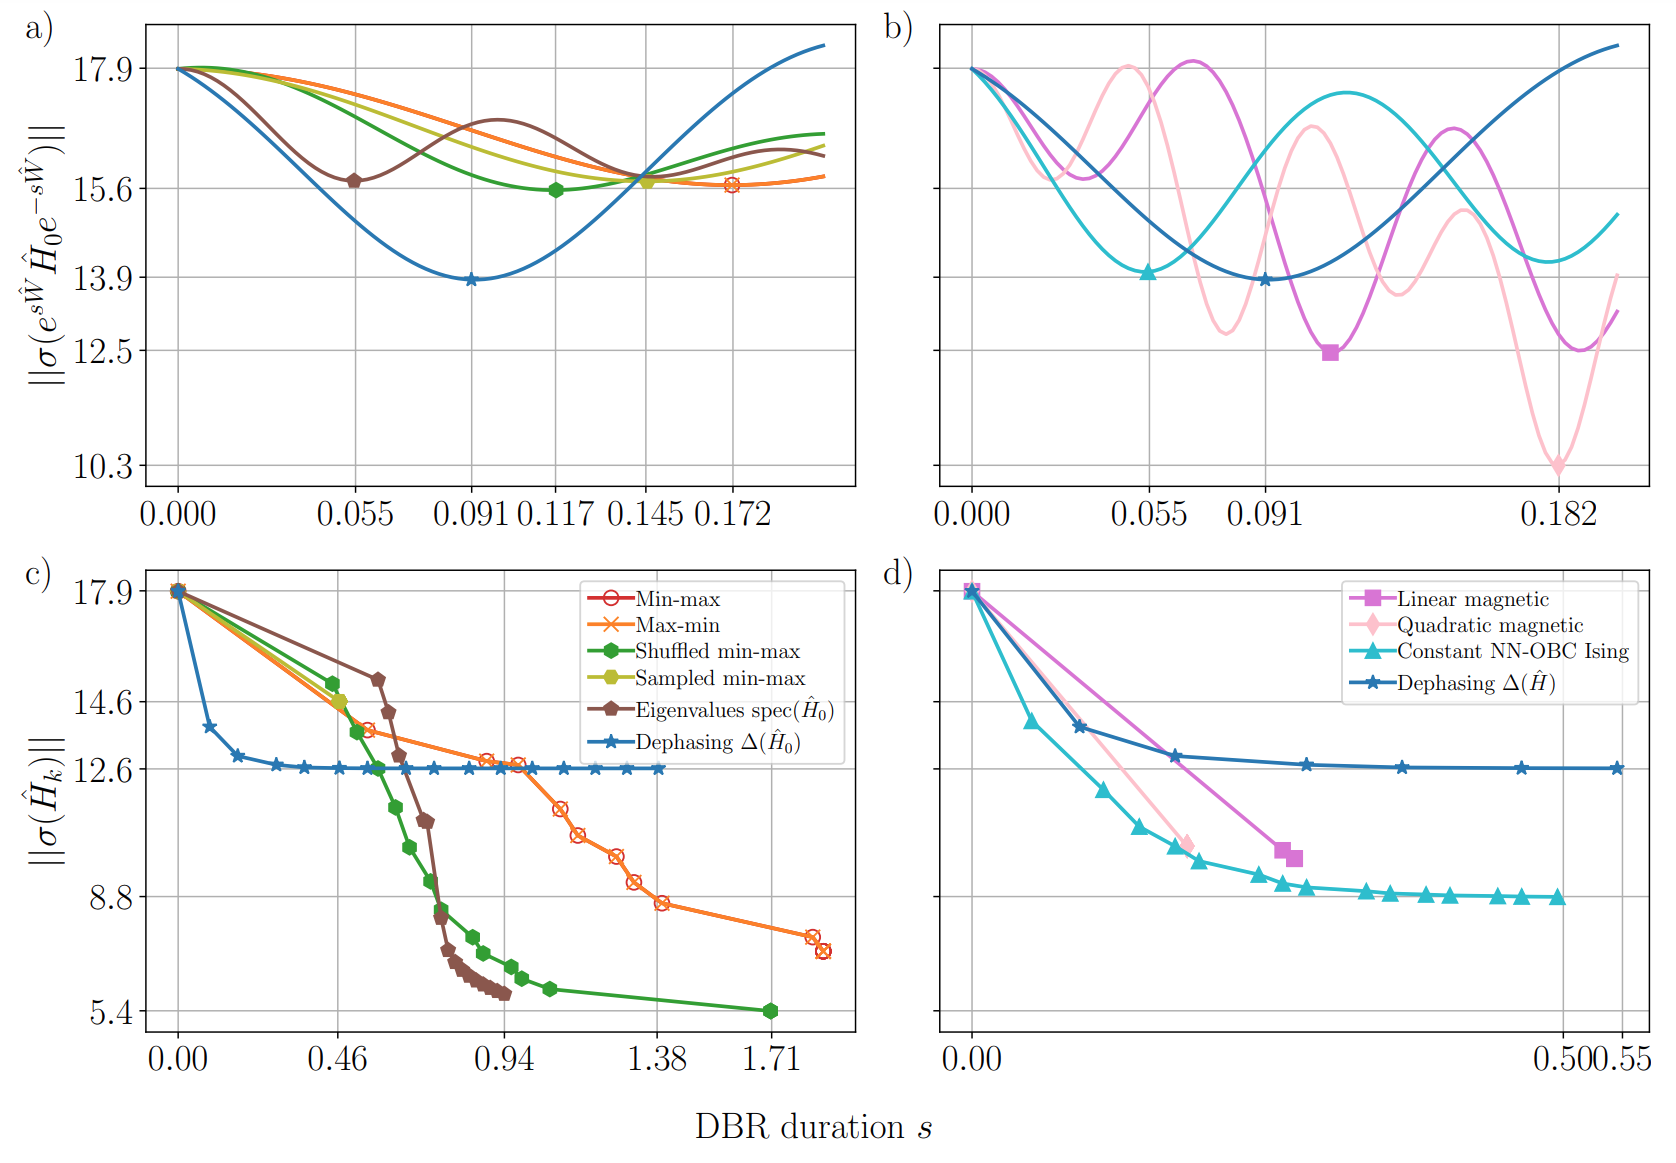
\includegraphics[width=0.6\textwidth]{figures/opt_strategies.png}
\end{figure}
\vspace{-0.2cm}
\begin{figure}
   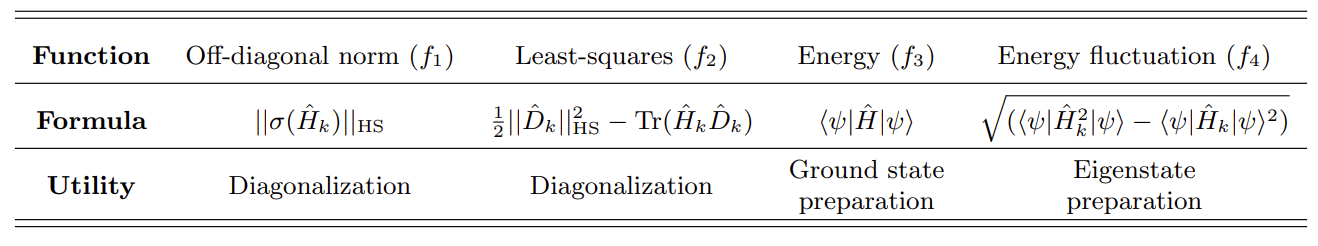
\includegraphics[width=0.7\textwidth]{figures/cost_functions.png}
\end{figure}
\begin{picture}(0,0)
    \put(335,150){
        
\includegraphics[width=0.15\textwidth]{figures/variational_icon.pdf}
    }
\end{picture}
\begin{picture}(0,0)
    \put(0,150){
        
\includegraphics[width=0.15\textwidth]{figures/analytical_icon.pdf}
    }
\end{picture}
\begin{picture}(0,0)
    \put(-20,40){
        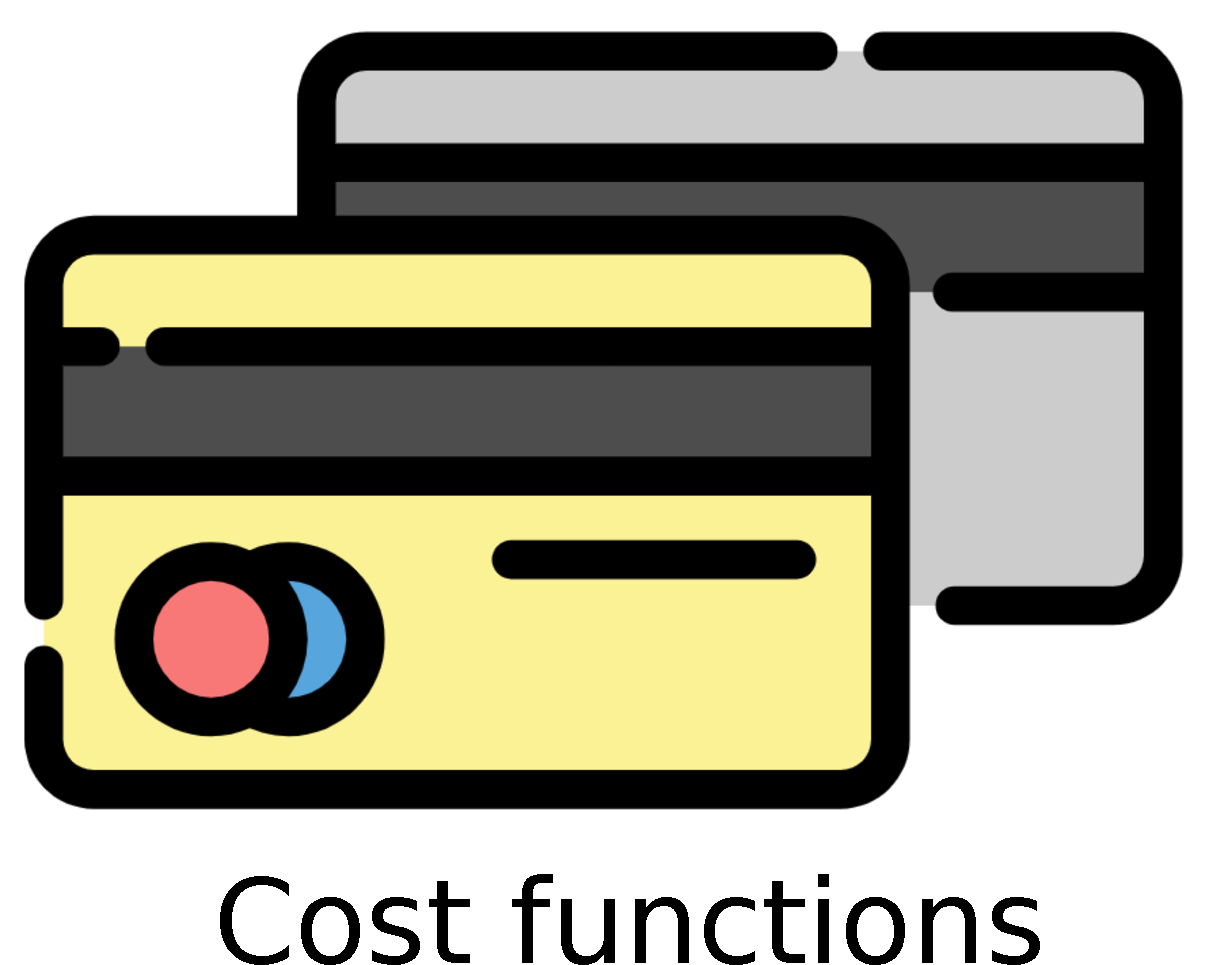
\includegraphics[width=0.15\textwidth]{figures/cost_icon.pdf}
    }
\end{picture}
\end{frame}

\begin{frame}{Double-bracket rotations can be optimized \hfill \href{https://arxiv.org/abs/2408.07431}{\textcolor{white}{\faBook\,\,arXiv:2408.07431}}}
\begin{center}
\begin{figure}
   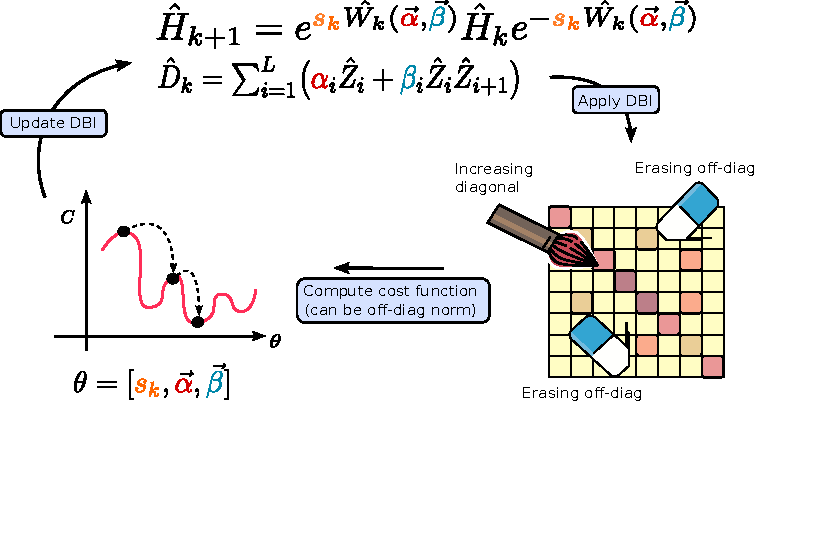
\includegraphics[width=1\textwidth]{figures/dbi_scheme_ink.pdf}
\end{figure}
\end{center}
\end{frame}

\begin{frame}{But how this can be a quantum algorithm? \hfill \href{https://arxiv.org/abs/2206.11772}{\textcolor{white}{\faBook\,\,arXiv:2206.11772}}}
The heart of the compilation of DBQAs is one of the \textbf{group commutator formulas} introduced
by Dawson and Nielsen in their \href{https://arxiv.org/abs/quant-ph/0505030}{Solovay-Kitaev algorithm}:
$$ \hat{V}^{\rm GC}(\hat{A}, \hat{B}) = e^{i\hat{A}} e^{i\hat{B}} e^{-i\hat{A}} e^{-i\hat{B}}, \qquad \qquad \hat{A}, \hat{B} \,\,\text{hermitian},$$
by means of which:
$$ e^{-[\hat{A}, \hat{B}]} = \hat{V}^{\rm GC}(\hat{A}, \hat{B}) + \hat{E}^{\rm GC}, $$
where 
$$  \hat{E}^{\rm GC} \leq \| [ \hat{A}, [\hat{A}, \hat{B}]] \| + \| [ \hat{B}, [\hat{B}, \hat{A}]] \|$$
in any unitarily invariant norm (e.g. Hilbert-Schmidt norm).

\begin{tcolorbox}[colback=red!15, title=How about DBI?]
$$ e^{- s [\hat{D}_0, \hat{H}_0]} = e^{i \sqrt{s_0}\hat{H}_0} 
e^{-i \sqrt{s_0}\hat{D}_0} e^{-i \sqrt{s_0}\hat{H}_0} e^{i \sqrt{s_0}\hat{D}_0} + O(s_0^{3/2}).$$
This is compilable into a sequence of local Hamiltonian evolutions.
\end{tcolorbox}
\faExclamationCircle\,\,Higher-order formulas can be implemented to reduce the approximation error.
\end{frame}

\begin{frame}{Sum up}
\begin{figure}
   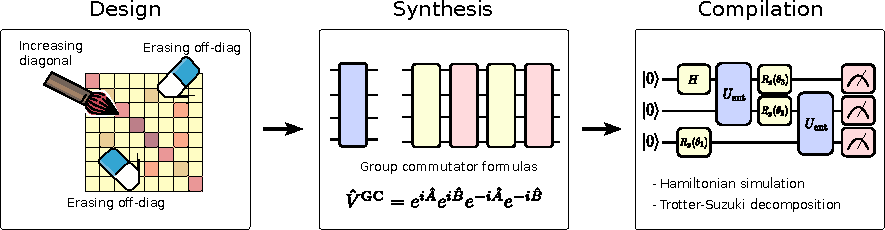
\includegraphics[width=1\textwidth]{figures/3_phases_dbqa.pdf}
\end{figure}
\end{frame}

\end{document}




